\chapter{Introducing new capabilities}\label{chap:chap4}

\epigraph{``If debugging is the process of removing software bugs, then programming must be the process of putting them in.''}{\textit{Edsger W. Dijkstra}}

\paragraph{}
In this chapter we will describe all the major additions that have been made to Arm's simulator. We will focus on discussing the changes that have introduced new functionalities, whereas the ones that were limited to refactoring the code without modifying its logic will only be briefly mentioned. This chapter can be logically divided into three parts: the work done to finish introducing all of the integer-based instructions, the implementation of the floating-point logic, and the necessary updates to the UI of the web application.

\section{Finishing the integer job}\label{chap:chap4int}
\paragraph{}
As was briefly mentioned in Chapter \ref{chap:chap1insidelook}, the simulator's logic is actually quite well structured and extensible when dealing with integer instructions, since the developers tailored everything, from the format of the instructions to the data structure of the registers, to work using integers. From this aspect, adding the remaining integer-based instructions to the simulator has been a simple work of extending the logic with new mnemonics and branches. However, some issues presented themselves due to some quirks of the Java language, which made implementing some instructions not as straightforward as it could have been.
\subsection{The logic around integer instructions}
\paragraph{}
Before exploring the individual instructions, we first need to explain the work necessary to introduce them to the pre-existing logic. The simulator has a few places where instructions are read, parsed, decoded, created and executed, and as such, when adding a new instruction, they have to be extended.
\paragraph{}
First of all, to introduce a new instruction we must first define its representation, meaning its mnemonic, encoding, and type. This is done inside the \verb|Mnemonic.java| class. As we can see from an excerpt in Listing \ref{lst:mnemonics}, we need to provide both the uppercase and the lowercase mnemonic for the instruction, its type (in this example, \verb|RRR| for instructions that operate on three registers, \verb|RRI| for ones that operate on two registers and one immediate value), and its encoding (usually the one provided in the textbook \cite{patterson2016computer} as shown in Figure \ref{fig:legv8instrlist}).
\begin{lstlisting}[float, caption={How mnemonics are defined}, label={lst:mnemonics}]
public enum Mnemonic {
  ADD("ADD", "add", TokenType.MNEMONIC_RRR, "10001011000"),
  ADDS("ADDS", "adds", TokenType.MNEMONIC_RRR, "10101011000"),
  ADDI("ADDI", "addi", TokenType.MNEMONIC_RRI, "1001000100"),
  ...
}
\end{lstlisting}
\paragraph{}
It is now the turn of the \verb|Decoder.java| class. As was detailed in the overview of the codebase, this is the class responsible for taking a line of parsed LEGv8 code and creating the actual instruction as defined in \verb|Instruction.java|. As we can see from Listing \ref{lst:instr}, this is done through a switch case by analyzing the mnemonic and instantiating the instruction with the given parameters.
\begin{lstlisting}[float, caption={The creation of instructions}, label={lst:instr}]
public static Instruction getInstruction(...) {
  switch (mnemonic) {
    case ADD :
      return new Instruction(mnemonic, ...);
    case ADDS :
      return new Instruction(mnemonic, ...);
    case ADDI :
      return new Instruction(mnemonic, ...);
    ...
}
\end{lstlisting}
\paragraph{}
\verb|TokenType.java| contains the definition of the regular expression required to correctly tokenize the LEGv8 syntax. We can see from Listing \ref{lst:toktype}, that the mnemonic of the valid instruction needs to be reported both in uppercase and lowercase in the appropriate enum case and added to the regular expression string.
\begin{lstlisting}[float, caption={Validating the syntax with regular expressions}, label={lst:toktype}]
public enum TokenType {
  // The order in which these enums are defined is important to get the longest RegExp match
  LBRACKET("\\[", 1, "["),
  RBRACKET("\\]", 2, "]"),
  ...
  REGISTER("[Xx][12][0-9]|[Xx]30|[Xx][0-9]|XZR|xzr|SP|sp|LR|lr|FP|fp|IP[01]|ip[01]", 5, "REGISTER"),
  ...
  MNEMONIC_RRI("ADDIS?[ \t]+|SUBIS?[ \t]+|..."),
  MNEMONIC_RRR("ADDS?[ \t]+|SUBS?[ \t]+|..."),
  ...
}
\end{lstlisting}
\paragraph{}
Finally, it comes time to implement the instruction's logic into \verb|CPU.java|. As we can see from an example in Listing \ref{lst:cpuinstr}, this is done by adding a new method with the appropriate arguments, and adding a case to the switch governing which instructions get executed. 
\begin{lstlisting}[float, caption={How an instruction is executed}, label={lst:cpuinstr}]
private void execute(Instruction ins, Memory memory) {
  switch (ins.getMnemonic()) {
    case ADD :
      ADD(args[0], args[1], args[2]);
      break;
  }
}
private void ADD(int destReg, int op1Reg, int op2Reg) {
  registerFile[destReg] = registerFile[op1Reg] + registerFile[op2Reg];
}
\end{lstlisting}
\paragraph{}
When implementing integer-based instructions, these are the necessary surrounding changes that need to be performed. Since the process has been now explained, from now on, in this section, we will focus only on the methods added to \verb|CPU.java|.
\subsection{MUL}
\paragraph{}
Multiplicative operations between two 64-bit numbers can end up giving a 128-bit result ($2^{64}\cdot2^{64}=2^{64+64}=2^{128}$). Since LEGv8 doesn't support 128-bit registers, how is multiplication handled? The \verb|MUL| instruction performs the product between two integers and simply writes the lower 64-bits of the multiplication to the destination register. In this case, the multiplication algorithm works the same for signed and unsigned values: if the result stays inside the 64-bit bounds, then no 128-bit extension is required and thus the sign is maintained, and if the result gets truncated then its sign is meaningless without the context of the higher 64 bits. Since Java automatically truncates the multiplication between integers the same way, it is easily implemented as can be seen from Listing \ref{lst:mul}.
\begin{lstlisting}[float, caption={Implementation of the MUL instruction}, label={lst:mul}]
private void MUL(int destReg, int op1Reg, int op2Reg) {
  registerFile[destReg] = registerFile[op1Reg] * registerFile[op2Reg];
}
\end{lstlisting}
\subsection{SMULH}
\paragraph{}
This instruction, again, multiplies together the values inside two \verb|X| registers, but in this case writes to the destination the higher 64 bits of the result, interpreting them as a signed multiplication.  When multiplying two 64-bit numbers, if we care about the higher 64 bits, they have to be both extended to 128 bits, and this extension operation needs to be aware if they are signed or unsigned for it to be performed correctly. In this case, we specify that the two values are signed. Here we encounter a limitation of Java's primitive integer types. Namely, they can be at most 64 bits long and their multiplication gets truncated just like with \verb|MUL|. For this reason, we need a way to perform products with signed integer values bigger than 64 bits. Here, Java's \verb|BigInteger.java| library and GWT's support for it come to the rescue, as they allow us to create arbitrarily wide signed integer numbers. As we can see from Listing \ref{lst:smulh}, we just need to convert the two 64-bit \verb|long| values into a \verb|BigInteger| and then use the provided \verb|multiply()| method to obtain the result. After this is done, we shift the higher 64 bits to the lower ones, and we convert it to a \verb|long| value to be written to the destination register.
\begin{lstlisting}[float, caption={Implementation of the SMULH instruction}, label={lst:smulh}]
private void SMULH(int destReg, int op1Reg, int op2Reg) {
  BigInteger fullResult = BigInteger.valueOf(registerFile[op1Reg].multiply(BigInteger.valueOf(registerFile[op2Reg]));
  BigInteger shiftedResult = fullResult.bitLength() > 64 ? fullResult.shiftRight(64) : BigInteger.valueOf(0);
  registerFile[destReg] = shiftedResult.longValue();			
}
\end{lstlisting}
\subsection{UMULH}
\paragraph{}
Following the prototype of the \verb|SMULH| instruction, \verb|UMULH| performs the same operation but interpreting the multiplication as unsigned. The logic is largely unchanged, except for another limitation of the Java language. Java does not have dedicated types for unsigned integers, both in the case of \verb|BigInteger| and of primitive types. This means that to perform an unsigned multiplication, we need a workaround to represent unsigned values as signed ones in such a way to obtain the correct results using the provided signed operations. This can be achieved, in this case,  by applying a particular bitmask \cite{web:bitmask} as defined in Listing \ref{lst:umulh}. This bitmask is used to convert 64-bit unsigned values into 65-bit signed ones in order to perform the correct multiplication. Even though the bits inside the register have no inherent interpretation, Java can only deal with signed \verb|long| values, and as such tricks such as these are needed to make it work. The rest of the operations are analogous to \verb|SMULH| case.
\begin{lstlisting}[float, caption={Implementation of the UMULH instruction}, label={lst:umulh}]
BigInteger UNSIGNED_LONG_MASK = |BigInteger.ONE.shiftLeft(Long.SIZE).subtract(BigInteger.ONE)|;
...
private void UMULH(int destReg, int op1Reg, int op2Reg) {
  BigInteger fullResult = BigInteger.valueOf(registerFile[op1Reg]|.and(UNSIGNED_LONG_MASK)|.multiply(BigInteger.valueOf(registerFile[op2Reg])|.and(UNSIGNED_LONG_MASK)|);
  BigInteger shiftedResult = fullResult.bitLength() > 64 ? fullResult.shiftRight(64) : BigInteger.valueOf(0);
  registerFile[destReg] = shiftedResult.longValue();
}
\end{lstlisting}
\subsection{SDIV}
\paragraph{}
This instruction performs the signed integer division between two 64-bit values. Since Java natively works using signed values and it doesn't automatically cast divisions between integers as floating-point, Listing \ref{lst:sdiv} shows the elementary implementation of the instruction.
\begin{lstlisting}[float, caption={Implementation of the SDIV instruction}, label={lst:sdiv}]
private void SDIV(int destReg, int op1Reg, int op2Reg) {
  registerFile[destReg] = registerFile[op1Reg] / registerFile[op2Reg];
}
\end{lstlisting}
\subsection{UDIV}
\paragraph{}
This instruction performs the unsigned integer division between two 64-bit values. As has already been mentioned, because of Java's limitations regarding unsigned integer values, we have to, again, use the bitmask in Listing \ref{lst:umulh} to represent unsigned values as signed. Thankfully, \verb|BigInteger| already provides a method for performing signed division, and Listing \ref{lst:udiv} shows the simple steps needed after the conversion is performed.
\begin{lstlisting}[float, caption={Implementation of the UDIV instruction}, label={lst:udiv}]
private void UDIV(int destReg, int op1Reg, int op2Reg) {
  BigInteger dividend = BigInteger.valueOf(registerFile[op1Reg]|.and(UNSIGNED_LONG_MASK)|;
  BigInteger divisor = BigInteger.valueOf(registerFile[op2Reg]|.and(UNSIGNED_LONG_MASK)|;
  BigInteger quotient = dividend.divide(divisor);
  registerFile[destReg] = quotient.longValue();
}
\end{lstlisting}
\subsection{LDA}
\paragraph{}
The last integer-based instruction that needs to be implemented is \verb|LDA|, which is actually a pseudo-instruction. Its purpose is to copy the address pointed by a label into an \verb|X| register. Since the instruction follows the same format as \verb|CBZ| and \verb|CBNZ| (i.e., its arguments are an \verb|X| register and a label), it was added as an \verb|RL|-type instruction. We should note that the LEGv8 documentation seems to be inconsistent in its description of this instruction. If we go by how it is used in the textbook's \cite{patterson2016computer} examples, it appears to do what we have described above. Instead, when looking at the LEGv8 Quick Reference Guide, it's described as \verb|R[Rd] = R[Rn] + DTAddress|, implying that it actually operates by taking the value of a register \verb|Rn|, adding it to the address \verb|DTAddress| specified by the label, and then writing the result into the \verb|Rd| destination address. Furthermore, this instruction is present in just a couple of LEGv8 examples and never explained in detail, so we decided to implement it following the code examples in the book instead of its specification, as can be seen in Listing \ref{lst:lda}.
\begin{lstlisting}[float, caption={Implementation of the LDA pseudo-instruction}, label={lst:lda}]
private void LDA(int destReg, long addressToLoad) {
  registerFile[destReg] = addressToLoad;
}
\end{lstlisting}
\section{Introducing floating-point capabilities}\label{chap:chap4float}
\paragraph{}
Both Java and LEGv8 support single-precision and double-precision operations following the IEEE-754 standard \cite{ieee754}, making it easy to transpose them from one another. Because of the simplicity of the code that will be presented when showcasing the new instructions, it has been chosen to group them together by type and precision to make the exposition less verbose. More complicated, though, are the steps that were needed to adapt the original codebase to make use of floating-point values and functions. This will our next topic of discussion.
\subsection{Setting the stage for the floating-point logic}
\paragraph{}
In the previous section, we have given a brief overview of the places in the codebase where integer instructions are dealth with, and as such where one needs to look for when trying to add new ones. Although similar steps need to be taken with floating-point instructions, some changes need to be made to previously untouched parts of the simulator to open the doors to floating-point instructions.
\paragraph{}
Floating-point instructions need floating-point registers, namely \verb|S| and \verb|D| registers. Fortunately, \verb|S| registers do not exist hardware-wise, as they are simply a way of referring to the lower 32 bits of the \verb|D| registers. Nonetheless, these additions require a change in how registers are represented. If before, inside of \verb|CPU.java|, they were a simply array of \verb|long|s, now a new type is needed to encapsulate their logic. For this, the \verb|Register.java| class and the \verb|RegisterType.java| enum class have been created, their content being presented in Listing \ref{lst:registerclass} and \ref{lst:registertypeclass} respectively.
\begin{lstlisting}[float, caption={The register class}, label={lst:registerclass}]
public final class Register {
  private final RegisterType type;
  private final int size;
  private long content;
  public Register(RegisterType type) {
    this.type = type;
    switch(type) {
      case X:
      case D: this.size = Memory.DOUBLEWORD_SIZE;
        break;
      case S: this.size = Memory.WORD_SIZE;
        break;
      default: this.size = Memory.DOUBLEWORD_SIZE;
  }
    content = 0L;
  }
  public void writeDoubleWord(long bits) {
    this.content = bits;
  }	
  public long readDoubleWord() {
    return this.content;
  }	
  public void writeWord(int bits) {
    this.content = (this.content & 0xffffffff00000000L) OR (bits & 0x00000000ffffffffL);
  }
  public int readWord() {
    return (int) this.content;
  }
  public RegisterType getType() {
    return type;
  }
  public int getSize() {
    return size;
  }
}
\end{lstlisting}
\begin{lstlisting}[float, caption={The RegisterType class}, label={lst:registertypeclass}]
public enum RegisterType {
  X, S, D
}
\end{lstlisting}
As can be seen, registers are now written to and read from using dedicated method calls, which also allows to transparently write 32-bit values to the lower bits.
\paragraph{}
After performing this change, \verb|CPU.java| now needs to hold two arrays, one of \verb|X| registers, and one of \verb|D| registers (with \verb|S| registers being included for free). This is shown in Listing \ref{lst:newregscpu}.
\begin{lstlisting}[float, caption={The new registers}, label={lst:newregscpu}]
...
private Register[]	XRegisterFile;
private Register[]	DRegisterFile;
...
/**
 * @param index	the register whose value to return, an integer in the range 0-31
 * @return		the value stored in the register <code>index</code>
 */
public long getRegister(RegisterType type, int index) {
  switch(type) {
    case X: return XRegisterFile[index].readDoubleWord();
    case D: return DRegisterFile[index].readDoubleWord();
    case S: return DRegisterFile[index].readDoubleWord() & 0x00000000ffffffffL;
    default: return 0L;
    }
}
\end{lstlisting}
We can also see that a new way of obtaining the values of the registers needed to be introduced to separate their type. In Listing \ref{lst:regaccref} we can see an example of how the rest of the code was refactored following these changes.
\begin{lstlisting}[float, caption={The refactored register access}, label={lst:regaccref}]
private void ADD(int destReg, int op1Reg, int op2Reg) {
  XRegisterFile[destReg]|.writeDoubleWord(|XRegisterFile[op1Reg]|.readDoubleWord()| + XRegisterFile[op2Reg]|.readDoubleWord())|;
}
\end{lstlisting}
\paragraph{}
The \verb|Decoder.java| class does not deal with the type of operations being performed. Its only interest is the amount of arguments each instruction takes. Since floating-point instructions follow the same structure as integer ones, adding them to this class followed the same procedure previously described. The only addition has been creating a new method shown in Listing \ref{lst:decoderrargs}.
\begin{lstlisting}[float, caption={New decoder for floating-point comparisons}, label={lst:decoderrargs}]
private static int[] decodeRRArgs(ArrayList<String> args) {
  int[] operands = new int[2];
  operands[0] = decodeRegister(args.get(0));
  operands[1] = decodeRegister(args.get(1));
  return operands;
}
\end{lstlisting}
Unlike with integer comparisons, floating-point ones are not an alias for the \verb|SUBS| or \verb|SUBIS| instructions. For this reason they are the only ones to truly operate on just two registers. This case needed to be added to the decoder.
\paragraph{}
Major changes needed to be performed on the \verb|TokenType.java| class. This is because, since LEGv8 prohibits hybrid instructions, it was necessary to impose that certain instructions only deal with certain registers and they cannot be mixed together. This made it necessary to create new types of TokenTypes for each register, and for each combination of instruction type and instruction format. An excerpt of this can be seen in Listing \ref{lst:tokentypenew} and can be compared with Listing \ref{lst:toktype}. Adding floating-point mnemonics is now analogous to adding integer ones, except they need to be put in the correct dedicated regular expression.
\begin{lstlisting}[float, caption={Refactoring of TokenType}, label={lst:tokentypenew}]
public enum TokenType {	
  LBRACKET("\\[", 1, "["),
  RBRACKET("\\]", 2, "]"),
  ...
  XREGISTER("[Xx][12][0-9]|[Xx]30|[Xx][0-9]|XZR|xzr|..."),
  SREGISTER("[Ss][12][0-9]|[Ss]30|[Ss][0-9]+", 6, "SREGISTER"),
  DREGISTER("[Dd][12][0-9]|[Dd]30|[Dd][0-9]+", 7, "DREGISTER"),
  ...
  XMNEMONIC_RRR("ADDS?[ \t]+|SUBS?[ \t]+|..."),
  SMNEMONIC_RRR("FADDS[ \t]+|FSUBS[ \t]+|..."),
  DMNEMONIC_RRR("FADDD[ \t]+|FSUBD[ \t]+|..."),
  ...
}
\end{lstlisting}
\paragraph{}
The change to \verb|TokenType.java| needed to be propagated to other classes making use of it. Firstly, \verb|Mnemonic.java| needed to be updated by refactoring all the integer instruction to follow the new \verb|TokenType|s. Regarding the addition of floating-point instructions, the procedure is now analogous to the integer ones, except they need to be given their dedicated argument type, as shown in Listing \ref{lst:mnemonicnew}.
\begin{lstlisting}[float, caption={Updated Mnemonic.java}, label={lst:mnemonicnew}]
public enum Mnemonic {
  ADD("ADD", "add", TokenType.XMNEMONIC_RRR, ...),
  ...
  FADDS("FADDS", "fadds", TokenType.SMNEMONIC_RRR, ...),
  FADDD("FADDD", "faddd", TokenType.DMNEMONIC_RRR, ...),
  ...
}
\end{lstlisting}
\paragraph{}
Secondly, the finite state machine in \verb|ParserState.java|, used to parse the tokens, needed to be integrated with all the new transitions it could take. This was achieved by mostly copying and adapting the existing transitions and adding them to the automata. Since hybrid instructions are not allowed, this meant simply adding new branches from the starting state, without making the logic more complex. Due to the verbosity of this class, a listing showcasing an excerpt of the changes is not provided.
\paragraph{}
Lastly, we haven't touched upon memory operations. This is because, even though the memory was designed with integer values in mind -- using \verb|long| or \verb|int| values -- this choice does not in fact hinder the introduction of floating-point values. Single and double-precision floating-point numbers are just 32 and 64-bit values which are given a certain interpretation. Since the memory does only care about storing raw bytes, we can keep using the existing logic by simply taking \verb|float| bits and turning them into \verb|int| bits when writing to the memory, and vice versa when reading. Same can be done between \verb|double| bits and \verb|long| bits. Java offers precisely these functionalities with the \verb|Float.floatToIntBits()| and \verb|Float.intBitsToFloat()|, and \verb|Double.doubleToLongBits()| and \verb|Double.longBitsToDouble()| respectively, and GWT implements them in its emulator. This also allows floating-point bits in the memory to be loaded into \verb|X| registers and be interpreted as integers and vice versa with \verb|S| and \verb|D| registers, which is part of the intended behavior. \verb|Float.floatToRawIntBits()| and \verb|Double.doubleToRawLongBits()| should be the preferred methods, but they aren't yet supported by GWT and they don't seem to cause any problems.
\paragraph{}
This concludes the changes inside the logic of the simulator that were needed to be performed in order to enable the addition and execution of the new floating-point instructions.
\subsection{FADDS, FDIVS, FMULS, FSUBS}
\paragraph{}
As was previously mentioned, implementing LEGv8's floating-point arithmetic in Java does not present the same problems as with integer operations. This is because they both follow IEEE-754's \cite{ieee754} specification and as such can be easily translated between each other. Listing \ref{lst:newfloatinstr} provides the code for \verb|FADDS|, \verb|FDIVS|, \verb|FMULS|, \verb|FSUBS|.
\begin{lstlisting}[float, caption={New single-precision arithmetic instructions}, label={lst:newfloatinstr}]
private void FADDS(int destReg, int op1Reg, int op2Reg) {
  DRegisterFile[destReg].writeWord(Float.floatToIntBits(
    Float.intBitsToFloat(DRegisterFile[op1Reg].readWord()) +
    Float.intBitsToFloat(DRegisterFile[op2Reg].readWord())
  ));
}
private void FSUBS(int destReg, int op1Reg, int op2Reg) {
DRegisterFile[destReg].writeWord(Float.floatToIntBits(
  Float.intBitsToFloat(DRegisterFile[op1Reg].readWord()) -
  Float.intBitsToFloat(DRegisterFile[op2Reg].readWord())
  ));
}
private void FMULS(int destReg, int op1Reg, int op2Reg) {
  DRegisterFile[destReg].writeWord(Float.floatToIntBits(
    Float.intBitsToFloat(DRegisterFile[op1Reg].readWord()) *
    Float.intBitsToFloat(DRegisterFile[op2Reg].readWord())
  ));
}
private void FDIVS(int destReg, int op1Reg, int op2Reg) {
  DRegisterFile[destReg].writeWord(Float.floatToIntBits(
    Float.intBitsToFloat(DRegisterFile[op1Reg].readWord()) /
    Float.intBitsToFloat(DRegisterFile[op2Reg].readWord())
  ));
}
\end{lstlisting}
\subsection{FADDD, FDVID, FMULD, FSUBD}
\paragraph{}
The same that has been said for single-precision arithmetic can be repeated verbatim in the case of double-precision. Listing \ref{lst:newdoubleinstr} presents the new double-precision instructions, following extremely close what was done in the single-precision case.
\begin{lstlisting}[float, caption={New double-precision arithmetic instructions}, label={lst:newdoubleinstr}]
private void FADDD(int destReg, int op1Reg, int op2Reg) {
  DRegisterFile[destReg].writeDoubleWord(Double.doubleToLongBits(
    Double.longBitsToDouble(DRegisterFile[op1Reg].readDoubleWord()) +
    Double.longBitsToDouble(DRegisterFile[op2Reg].readDoubleWord())
  ));
}
private void FSUBD(int destReg, int op1Reg, int op2Reg) {
  DRegisterFile[destReg].writeDoubleWord(Double.doubleToLongBits(
    Double.longBitsToDouble(DRegisterFile[op1Reg].readDoubleWord()) -
    Double.longBitsToDouble(DRegisterFile[op2Reg].readDoubleWord())
  ));
}
private void FMULD(int destReg, int op1Reg, int op2Reg) {
  DRegisterFile[destReg].writeDoubleWord(Double.doubleToLongBits(
    Double.longBitsToDouble(DRegisterFile[op1Reg].readDoubleWord()) *
    Double.longBitsToDouble(DRegisterFile[op2Reg].readDoubleWord())
  ));
}
private void FDIVD(int destReg, int op1Reg, int op2Reg) {
  DRegisterFile[destReg].writeDoubleWord(Double.doubleToLongBits(
    Double.longBitsToDouble(DRegisterFile[op1Reg].readDoubleWord()) /
    Double.longBitsToDouble(DRegisterFile[op2Reg].readDoubleWord())
  ));
}
\end{lstlisting}
\subsection{FCMPS, FCMPD}
\paragraph{}
When dealing with comparisons, the IEEE-754 standard \cite{ieee754} provides all the criteria for all the possible value combinations. The results must then be translated into LEGv8's control flags. The book \cite{patterson2016computer} does not include a table for floating-point flag-setting conventions like with integers in Figure \ref{fig:condjumpflags}. As such, we have chosen to use ARMv8's criteria \cite{web:armv8ieeejumpcodes} which are summarized in Figure \ref{fig:armv8condflags}.
\begin{figure}[H]
    \centering
    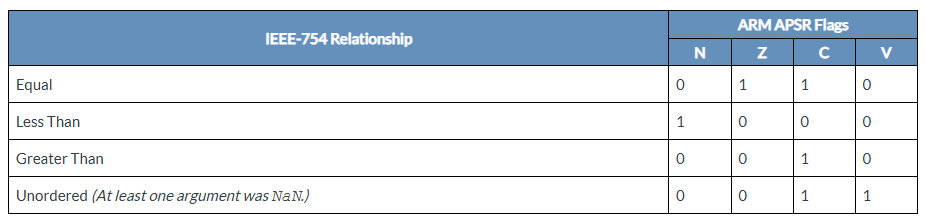
\includegraphics[width=1\linewidth]{img/ieee754_flags.png}
    \caption{ARMv8 floating-point condition flags. From \emph{Arm community blogs} \cite{web:armv8ieeejumpcodes}}
    \label{fig:armv8condflags}
\end{figure}
As we can see, both in the case of single and double-precision, the outcomes relate to the same flag values. For this reason a helper function called \verb|FCMPSetFlags| was created to work in both cases. As Listing \ref{lst:floatcmp} shows, both \verb|FCMPS| and \verb|FCMPD| use Java's built in floating-point comparison utilities and then pass the results to the helper function which sets the flags accordingly.
\begin{lstlisting}[float, caption={Floating-point comparisons implementations}, label={lst:floatcmp}]
private void FCMPSetFlags(int comparisonResult, boolean isNaN) {
  setNflag(comparisonResult < 0 && !isNaN);
  setZflag(comparisonResult == 0 && !isNaN);
  setCflag(comparisonResult >= 0 || isNaN);
  setVflag(isNaN);
}
...
private void FCMPS(int op1Reg, int op2Reg) {
  float op1f = Float.intBitsToFloat(DRegisterFile[op1Reg].readWord());
  float op2f = Float.intBitsToFloat(DRegisterFile[op2Reg].readWord());
  FCMPSetFlags(Float.compare(op1f, op2f), Float.isNaN(op1f) || Float.isNaN(op1f));	
}
private void FCMPD(int op1Reg, int op2Reg) {
  double op1d = Double.longBitsToDouble(DRegisterFile[op1Reg].readDoubleWord());
  double op2d = Double.longBitsToDouble(DRegisterFile[op2Reg].readDoubleWord());
  FCMPSetFlags(Double.compare(op1d, op2d), Double.isNaN(op1d) || Double.isNaN(op2d));
}
\end{lstlisting}
\subsection{STURS, LDURS}
\paragraph{}
Since the memory is type-agnostic, writing and reading from it can be done using \verb|int|s as representations for raw 32 bits, as can be seen in Listing \ref{lst:stursldurs}. Other than reading the lower 32 bits of \verb|D| registers, the logic is analogous to the integer load and store instructions.
\begin{lstlisting}[float, caption={Single-precision load and store instructions}, label={lst:stursldurs}]
private void STURS(int valReg, int baseAddressReg, int offset, Memory memory) {
  memory.storeWord(XRegisterFile[baseAddressReg].readDoubleWord()+offset, DRegisterFile[valReg].readDoubleWord());
  clearExclusiveAccessTag(XRegisterFile[baseAddressReg].readDoubleWord()+offset, Memory.DOUBLEWORD_SIZE);
}
private void LDURS(int destReg, int baseAddressReg, int offset, Memory memory) {
  DRegisterFile[destReg].writeWord((int) memory.loadDoubleword(XRegisterFile[baseAddressReg].readDoubleWord()+offset));
}
\end{lstlisting}
\subsection{STURD, LDURD}
\paragraph{}
Similarly, double-precision load and store operations use \verb|long|s as a neutral representation of raw 64 bits. They function the same way as single-precision and integer ones, as seen in Listing \ref{lst:sturdldurd}.
\begin{lstlisting}[float, caption={Double-precision load and store instructions}, label={lst:sturdldurd}]
private void STURD(int valReg, int baseAddressReg, int offset, Memory memory) {		 
  memory.storeDoubleword(XRegisterFile[baseAddressReg].readDoubleWord()+offset, DRegisterFile[valReg].readDoubleWord());
  clearExclusiveAccessTag(XRegisterFile[baseAddressReg].readDoubleWord()+offset, Memory.DOUBLEWORD_SIZE);
}
private void LDURD(int destReg, int baseAddressReg, int offset, Memory memory) {
  DRegisterFile[destReg].writeDoubleWord(memory.loadDoubleword(XRegisterFile[baseAddressReg].readDoubleWord()+offset));
}
\end{lstlisting}
\paragraph{}
This concludes the discussion of the changes made to the internal logic and behavior of the simulator. The following section will focus on the changes made to the UI and their motivations.

\section{UI additions and refinements}\label{chap:chap4UI}
\paragraph{}
It is clear from everything that has been discussed in this chapter and in Chapter \ref{chap:chap1outsidelook}, that the UI needs to undergo a few changes in order to incorporate all the new additions to the floating point logic, and to fix some of its shortcomings. This section will discuss the addition of the stack visualization, floating point registers, and the final reorganization of the UI elements.
\subsection{Visualizing the stack memory}
\paragraph{}
Having laid the work for the simulation of more complex programs with different types of data, being able to keep track of the state of the stack is of vital importance both for learning how the LEGv8 ISA works, and to debug more complex programs whose correct execution might not be evident from the registers' values alone.
\paragraph{}
If we take inspiration from how registers are visualized, we can see that they have a label, a signed integer or hexadecimal representation of their content, and a button to switch between the two. Even though the memory is addressed byte by byte, if we consider the fact that, usually, entire 64-bit values are loaded and stored, and the stack pointer only moves in quadword increments, it is more useful and intuitive to visualize the stack with panels each representing a doubleword worth of bytes, i.e. 8 bytes in LEGv8's case. The address referring to each doubleword can be considered the stack cell's label. The content, unlike with registers, does not have a preferred interpretation, therefore we can keep the raw hexadecimal one. Having done these considerations, it becomes obvious that an easy way to implement the visualization of the stack is to copy how it's done by the registers. For this reason, all that was needed was to take \verb|RegisterPanel.java| and slightly modify it to obtain \verb|StackPanel.java|, a representation of a single stack memory cell. In the \verb|WebApp.java| class, we just need to add an array of 32 \verb|StackPanel|s in descending order from the top of the stack, and group them into two columns just like with the registers, obtaining the end result shown in Figure \ref{fig:stackregs}.
\begin{figure}[H]
    \centering
    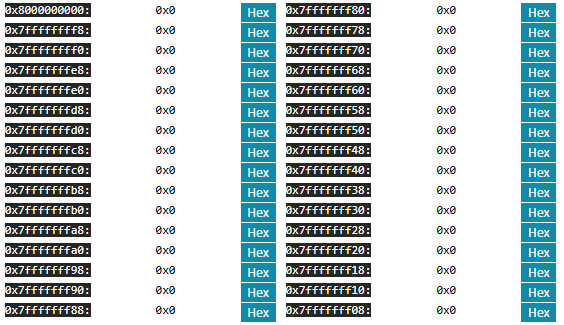
\includegraphics[width=0.85\linewidth]{img/stack_vis.png}
    \caption{The new stack visualization}
    \label{fig:stackregs}
\end{figure}
The values inside, instead of being updated with what's inside the registers, get updated at each cycle with the corresponding values in the stack. The code excerpt in Listing \ref{lst:stackpanelupd} shows how the stack panels are initialized and updated.
\begin{lstlisting}[float, caption={Stack panels' logic}, label={lst:stackpanelupd}]
private void initStackPanel() {
  HorizontalPanel stackFile = new HorizontalPanel();
  VerticalPanel leftStackPanel = new VerticalPanel();
  VerticalPanel rightStackPanel = new VerticalPanel();
  rightStackPanel.setHorizontalAlignment(HasHorizontalAlignment.ALIGN_CENTER);
  for (int i = 0; i < 32; i++) {
    stackPanels[i] = new StackPanel(Memory.STACK_BASE - i * 8);
    stackPanels[i].setStyleName("individualReg");
    if (i < 16) {
      leftStackPanel.add(stackPanels[i]);
    } else {
      rightStackPanel.add(stackPanels[i]);
    }
    }
    stackFile.add(leftStackPanel);
    stackFile.add(rightStackPanel);
    stackPanel = new VerticalPanel();
    stackPanel.addStyleName("registerPanel");
    stackPanel.add(stackFile);
    }
...
private void updateStackLabels(LEGv8_Simulator sim) {
  for (int i = 0; i < stackPanels.length; i++) {
    try {
      stackPanels[i].update(sim.getMemoryState().loadDoubleword(Memory.STACK_BASE - i * 8));
    } catch (SegmentFaultException e) {
        continue;
      }
    }
}
\end{lstlisting}
\subsection{Showing the floating-point registers}
\paragraph{}
Similarly, once floating-point capabilities were introduced, the respective visualization for the new floating-point registers needed to be added. In this case the parallels with integer registers are even stronger, and as such not even a new class was needed to implement this functionality. The only real difference, apart from the names on the labels, is the fact that floating-point values can be represented with the raw hexadecimal or with the decimal dotted notation. For this reason, the only changes made to how they work, as can be seen in Listing \ref{lst:floatregistersviz}, were regarding their labels and the functionality of their button. The final result can be seen in Figure \ref{fig:floatregsvis}.
\begin{figure}[H]
    \centering
    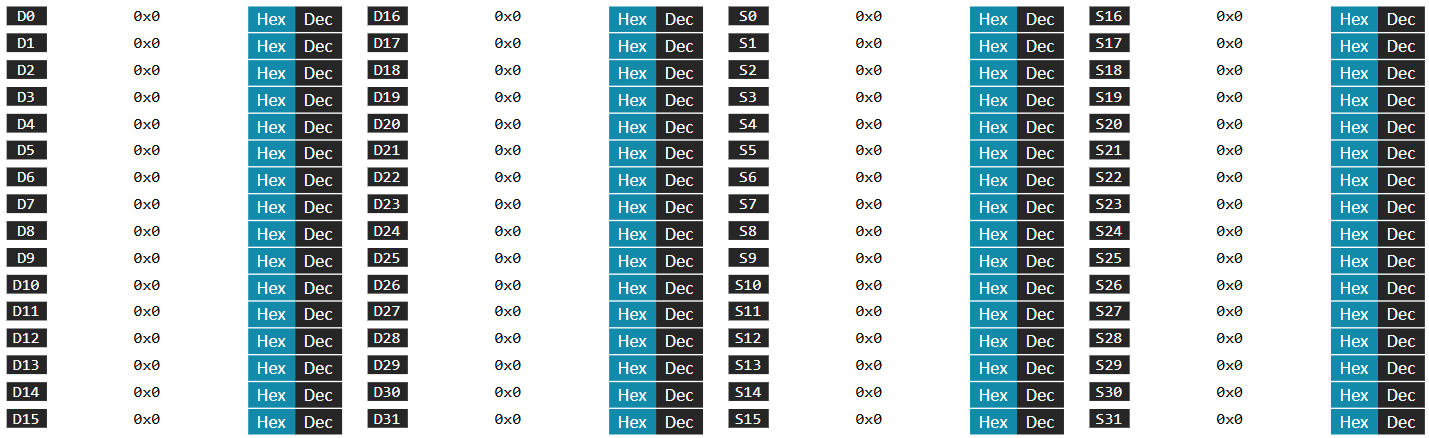
\includegraphics[width=1\linewidth]{img/float_regs_vis.png}
    \caption{The final floating point register panels visualization}
    \label{fig:floatregsvis}
\end{figure}
\begin{lstlisting}[float, caption={Logic of the floating-point registers' visualization}, label={lst:floatregistersviz}]
private void updateRegisterLabels(...) {
  for (int i = 0; i < XRegPanels.length; i++) {
    XRegPanels[i].update(getCPURegister(RegisterType.X, i));
  }
  for (int i = 0; i < DRegPanels.length; i++) {
    DRegPanels[i].update(getCPURegister(RegisterType.D, i));
  }
for (int i = 0; i < SRegPanels.length; i++) {
  SRegPanels[i].update(getCPURegister(RegisterType.S, i));
  }
  pcPanel.update(sim.getPC());
}
...
private String convertToDecimal() {
  switch(this.regType) {
    case X: return Long.toString(regValue);
    case D: return Double.toString(Double.longBitsToDouble(regValue));
    case S: return Float.toString(Float.intBitsToFloat((int) regValue));
    default: return "";
  }
}
\end{lstlisting}
\subsection{Reorganizing the UI}
\paragraph{}
The additions of the new UI elements discussed in the previous sections naturally entice a partial change in the design of the web page. Furthermore, as was pointed out in Chapter \ref{chap:chap1outsidelook}, one of the shortcomings of the UI is that it reacts poorly to changes in page size. Due to the complexity of GWT and the components used (such as AceGWT), it was chosen to simply freeze the UI and make it inert to resizing, meaning the page simply zooms in without rearranging anything. Although this fixed position approach might make things a bit more cumbersome for small screen users, at least it gives them the ability to move around the page or even zoom out while maintaining the correct proportions and element positions.
\paragraph{}
The first page to be reorganized is the Single Cycle visualization. To accommodate the newly introduced stack and floating-point register visualizations, they have been arranged as to fill the main page. The datapah visualization, although useful, is secondary to the simulation and occupied a lot of space. It has been chosen to put it below the main simulator interface, still reachable with a slight scroll down. Lastly, the CPU log panel, being there just for debugging purposes, has been put on the bottom of the page. Figure \ref{fig:newsimhomepage} presents this new look, which can be compared with the original in Figure \ref{fig:ogsimhomepage}.
\begin{figure}[]
    \centering
    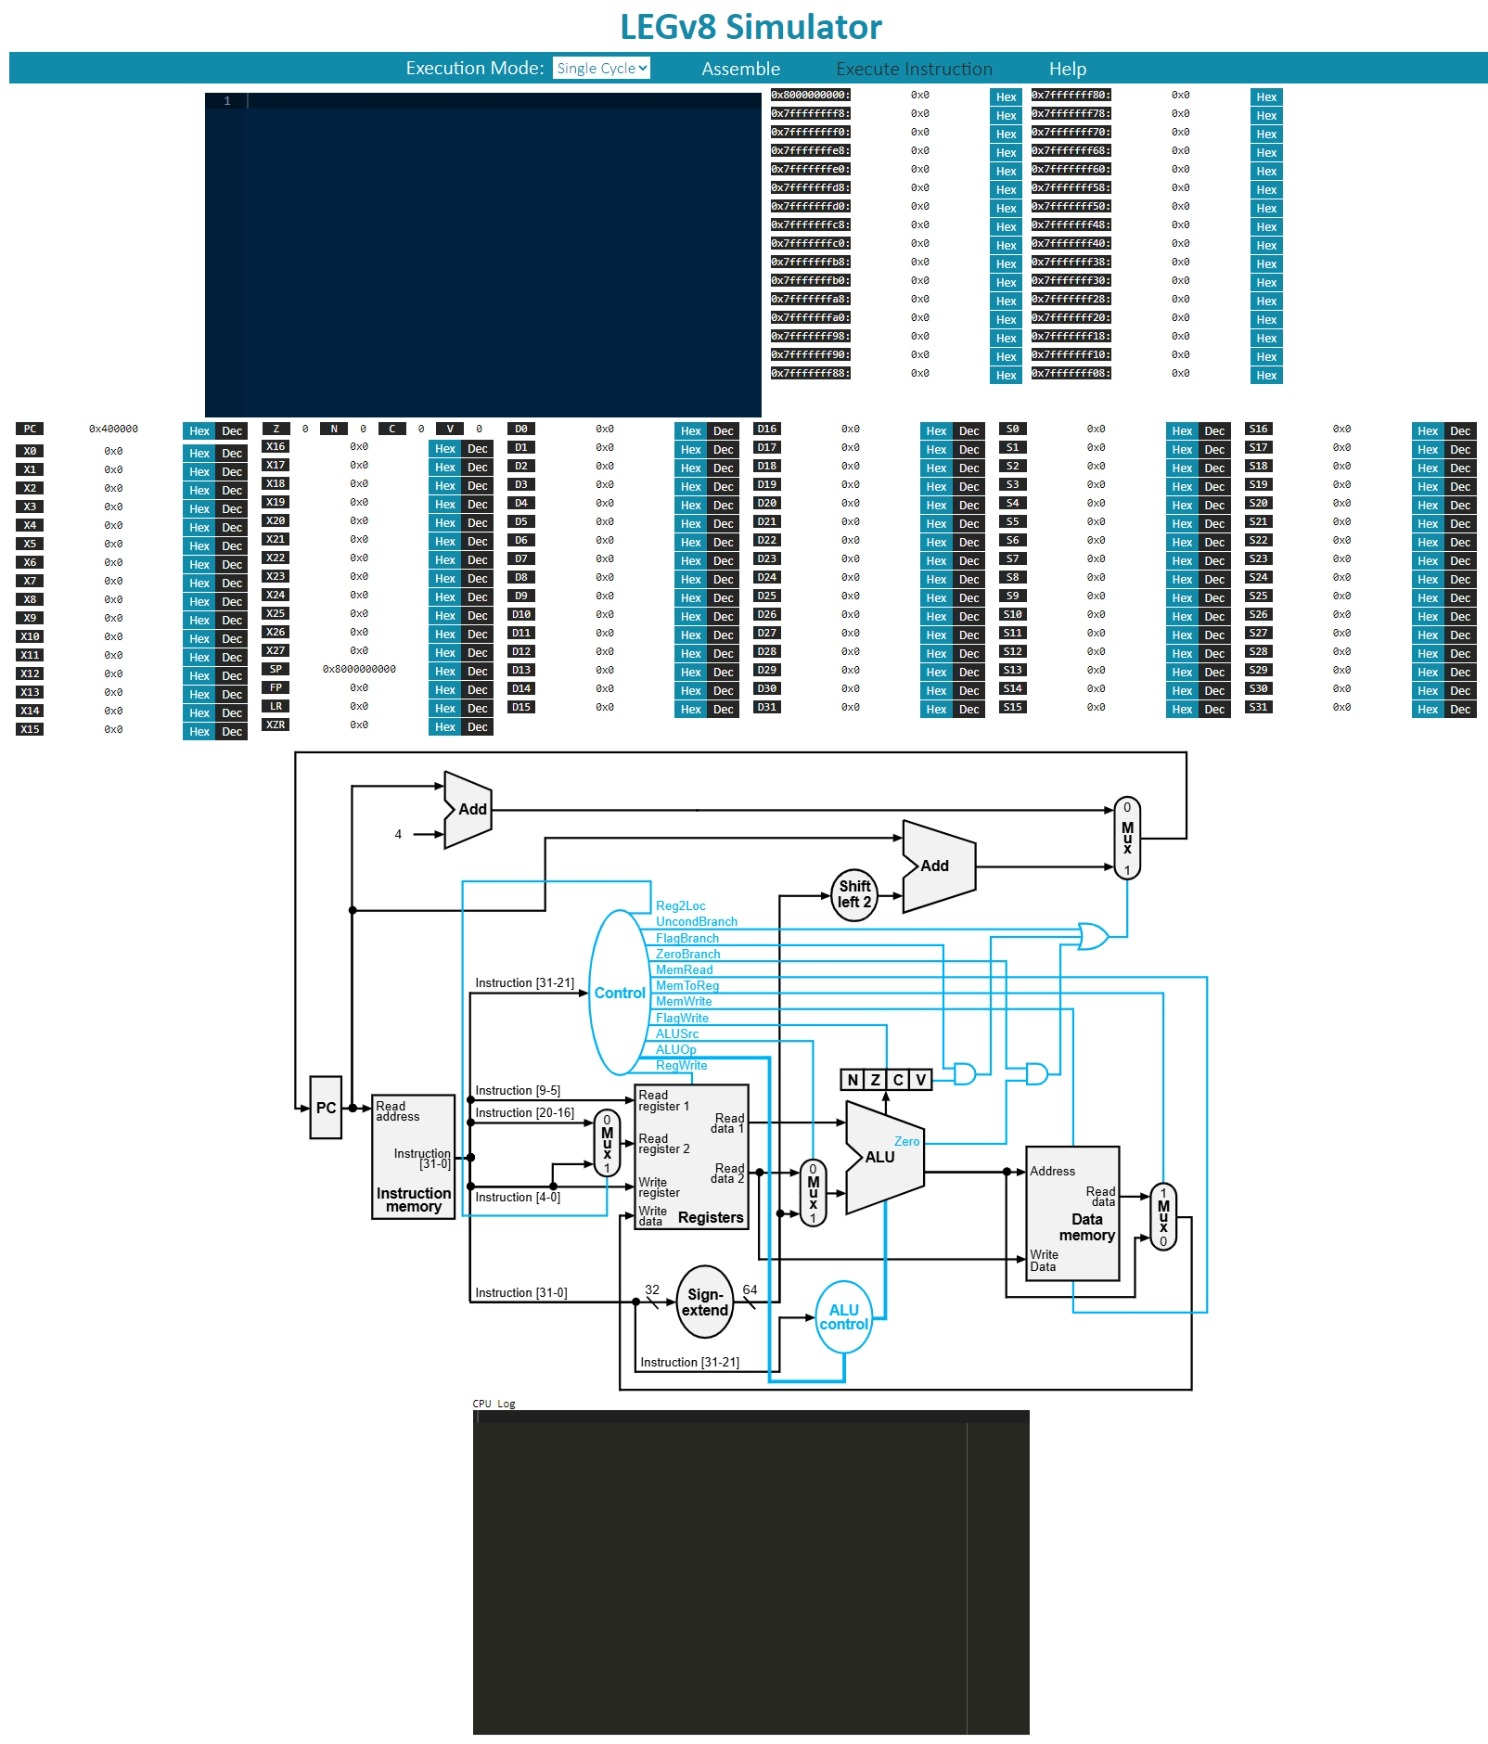
\includegraphics[width=1\linewidth]{img/new_single_cycle.jpeg}
    \caption{The updated Single Cycle visualization}
    \label{fig:newsimhomepage}
\end{figure}
\paragraph{}
Although the pipeline execution was not touched upon in this thesis' work, similar actions have been taken to enhance its look. When compared with Figure \ref{fig:ogpipelineview}, the updated UI puts, again,  the datapath visualization on the bottom, but moves the CPU log to the right of the stack panel. This is because, in the pipelined mode, the CPU log panel provides critical updates to the state of the pipeline, which is very important to keep visible in the main UI. Figure \ref{fig:newpipelinevis} showcases this new arrangement.
\begin{figure}
    \centering
    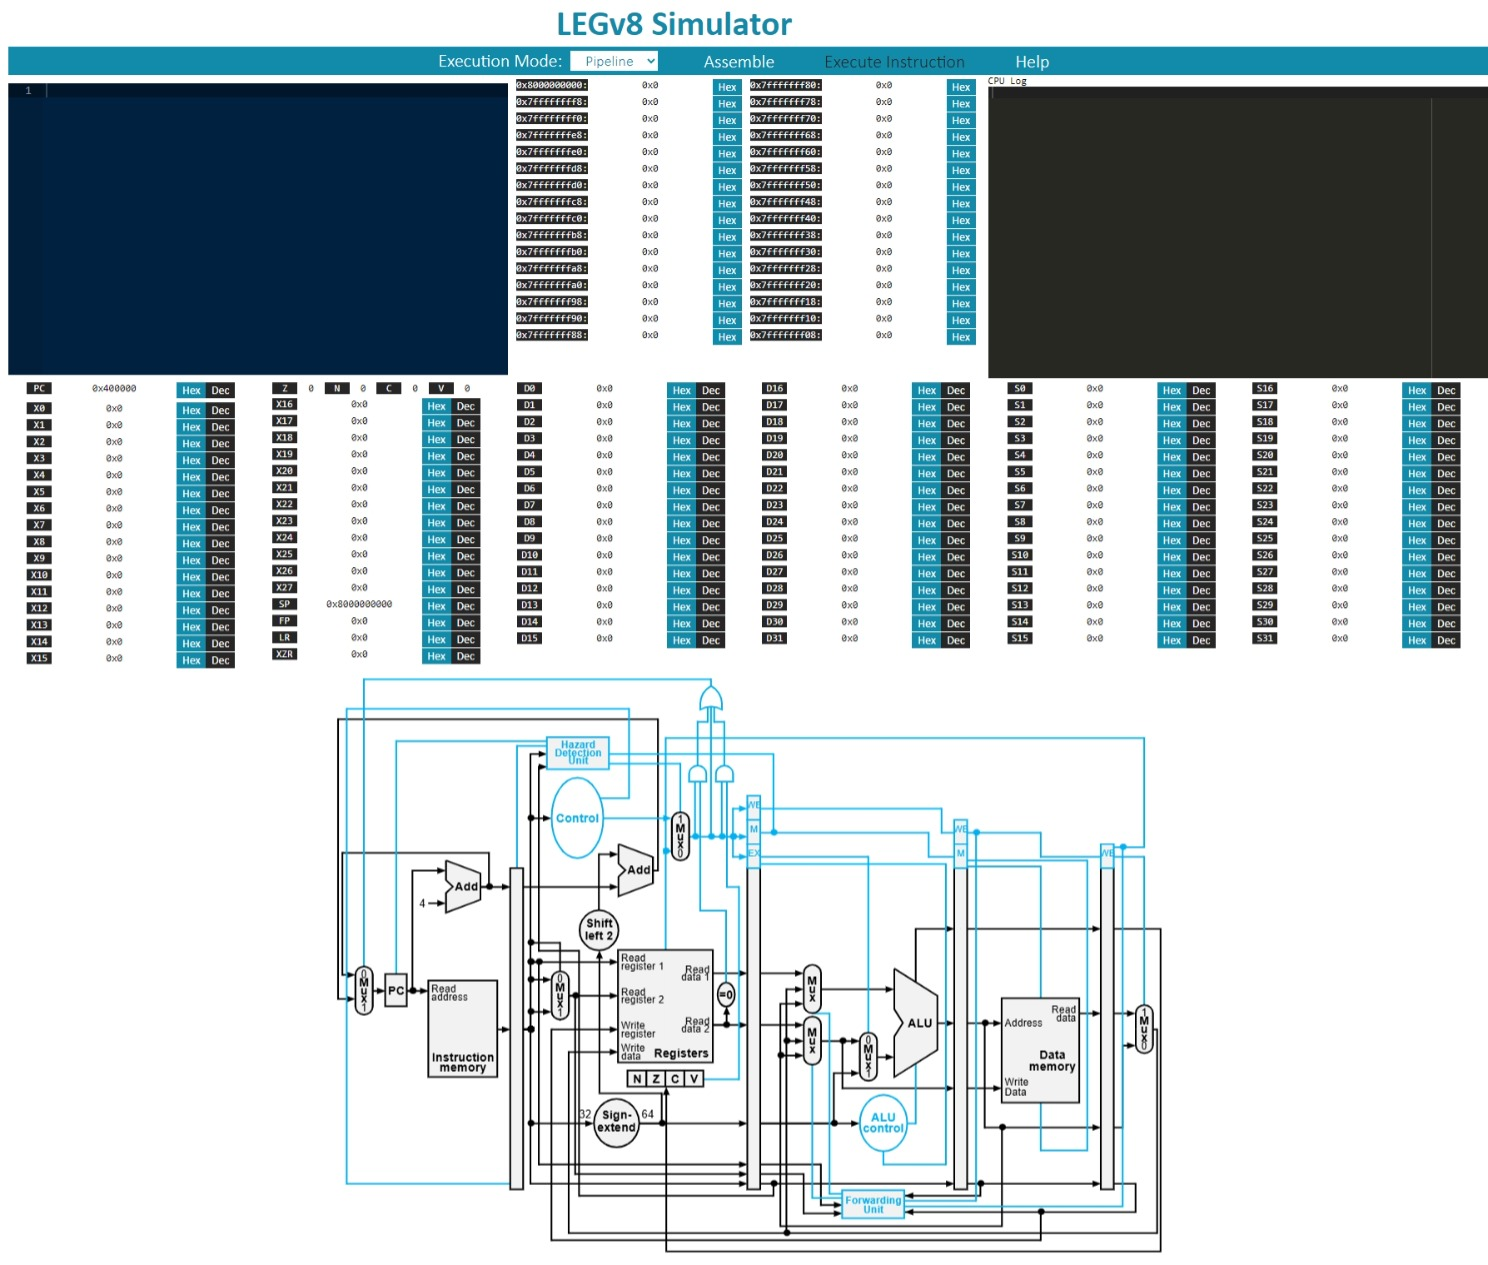
\includegraphics[width=1\linewidth]{img/new_pipeline.jpeg}
    \caption{The updated pipeline execution mode}
    \label{fig:newpipelinevis}
\end{figure}
\section{Conclusions}
\paragraph{}
In this chapter we have showcased the work done to fix, improve and implement new elements into the original simulator's web UI. Due to the design of the codebase, the process has been straightforward, in spite of GWT's quirky behavior. The end result is a more compact, featureful, informative UI which maintains the same visual language and appearence as the original. This concludes the work of this thesis. The next chapter will provide a summary of our efforts and an outlook on the future of the simulator.